% !TEX encoding = UTF-8
% !TEX program = pdflatex
% !TEX root = InformationRetrieval.tex
% !TEX spellcheck = it-IT

% 29 Settembre 2016

\chapter{Introduzione}

Lo scopo del reperimento dell'informazione è quello di essere in grado di soddisfare il bisogno informativo di una determinata categoria di utenti, mediante tecniche di ricerca e di memorizzazione dei dati.
Tali dati possono essere in qualsiasi formato: testo, foto, audio, ecc. e possono anche esserci problemi riguardo l'internazionalizzazione dei dati, legati all'utilizzo di lingue diverse.

Si ha quindi che c'è un utente che ha un'esigenza informativa che deve essere colmata reperendo delle informazioni da una collezione di documenti.

\section{Terminologia}

\begin{itemize}
	\item \textbf{Esigenza informativa}: mancanza di informazione che un utente vuole colmare per risolvere un suo problema e prendere delle decisioni.
	\item \textbf{Documento}: inteso come ``materializzazione'' dell'informazione, è un qualsiasi oggetto che contiene informazioni utili a soddisfare l'esigenza informativa.
	\item \textbf{Rilevanza}: proprietà di un ``documento'' di contenere l'informazione utile e necessaria a soddisfare una specifica esigenza informativa dell'utente.
	\item \textbf{Sistema di Reperimento dell'informazione}: sistema che a partire da una query e da un insieme di documenti, utilizza delle specifiche rappresentazioni per valutare la similarità tra i documenti e la query, in modo da fornire in risposta all'utente un insieme ordinato di documenti secondo un determinato ranking. Può esserci anche un sistema di feedback basato sulle preferenze dell'utente (assessment).
\end{itemize}


\section{Informazioni organizzative}

Orario delle lezioni

\begin{itemize}
	\item Giovedì dalle 10:30 - Aula Oe
	\item Venerdì dalle 12:30 - Aula Oe
\end{itemize}

Ci saranno degli homework che riguardano:
\begin{itemize}
	\item Un progetto individuale di valutazione di un sistema di reperimento dell'informazione. 
	\item Readings:  si studia uno o due articoli e si fa una presentazione stile seminariale.
\end{itemize}

Il ricevimento è per appuntamento.

Comunicazioni via mail a \url{maristella.agosti@unipd.it}, specificando come oggetto \texttt{[IR2016-2017]} e il nome/cognome/matricola.


\subsection{Modalità d'esame}

\begin{itemize}
	\item Esame scritto su tutto il programma svolto, da 0 a 20 punti, con sufficienza a 12.
	\item Progetto individuale di valutazione, da 0 a 5 punti.
	\item Readings, da 0 a 5 punti.
	\item Eventuale integrazione orale.
\end{itemize}

La pagina di riferimento del corso è \url{http://www.dei.unipd.it/~agosti/ir-2016-2017/}. 
C'è anche il corso sul Moodle del DEI: la password del corso è \texttt{corso-IR201617}.

Testi di riferimento:
\begin{itemize}
	\item Information Retrieval (2ed). Cornelis Joos. 1979. \url{http://www.dcs.gla.ac.uk/Keith/Preface.html}.
	\item Information Retrieval in Practice. W. Bruce Croft. 2010. \url{http://ciir.cs.umass.edu/irbook/}
\end{itemize}


\section{Programma e quadro d'insieme}

L'obiettivo del corso è quello di fornire le competenze necessarie per la ideazione, progettazione e implementazione di un sistema di reperimento dell'informazione.

Una parte importante del corso sarà dedicata all'indicizzazione: la parte del sistema che si occupa di gestire la rappresentazione dei documenti e della query dell'utente, specialmente per quanto riguarda l'ambito testuale.

Una volta effettuata l'indicizzazione viene definito un modello di valutazione che è la componente del sistema che si occupa di valutare la similarità tra la query e i documenti.

Il modello non è solo un algoritmo, ma c'è anche un insieme di costrutti che sono formalizzati allo scopo di rendere possibile la rappresentazione del contenuto dei documenti e delle interrogazioni. 

La valutazione del sistema si basa sull'efficacia e riguarda la coerenza che c'è tra i documenti reperiti e la richiesta dell'utente, così come ci sono metodi di valutazione per la parte legata all'indicizzazione e al modello.

\begin{figure}[htbp]
	\centering
	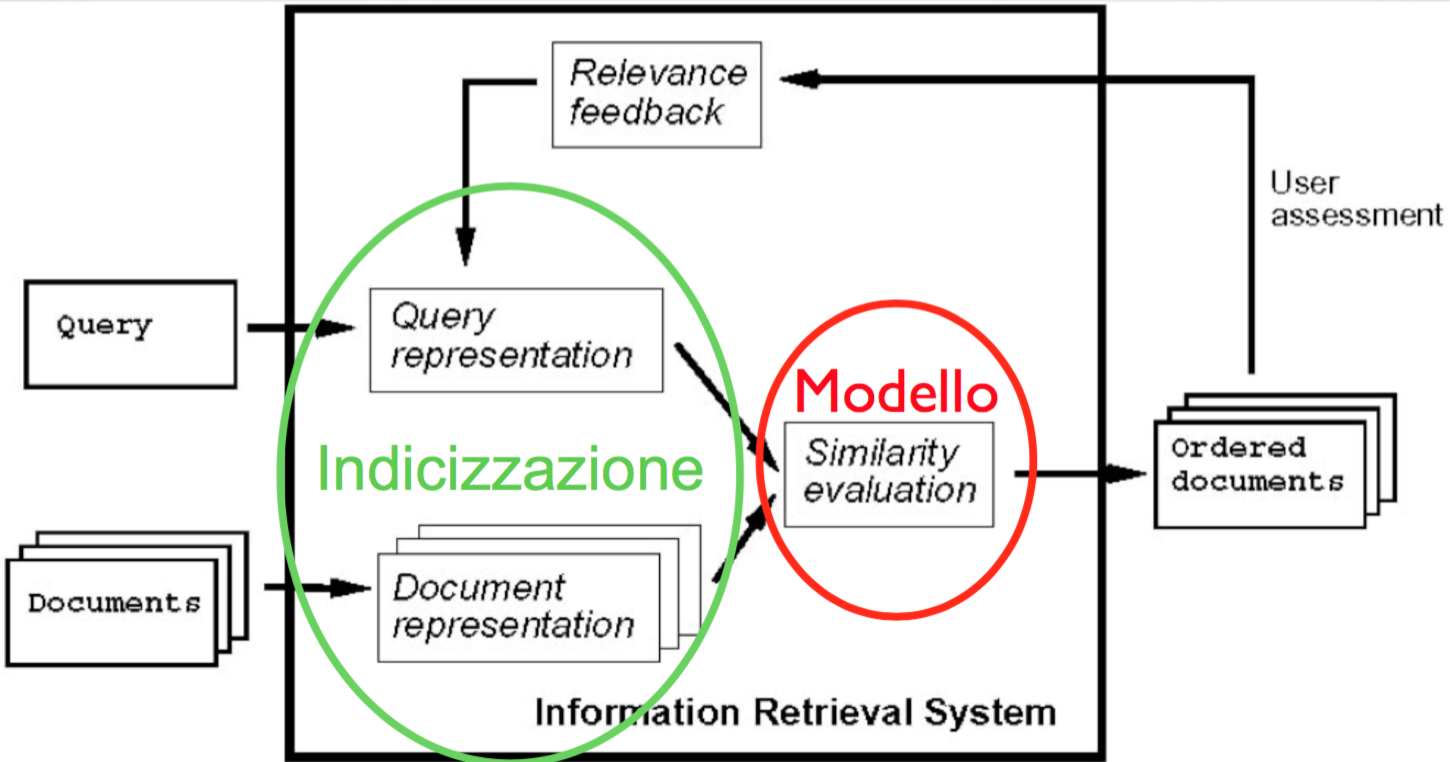
\includegraphics[width=.6\textwidth]{images/l1-irs.png}
	\caption{Sistema di Information Retrieval}
\end{figure}

\subsection{Programma}

\begin{itemize}
	\item Elementi introduttivi per la rappresentazione, gestione e reperimento automatico dell'informazione testuale.
	\item Indicizzazione: strutture dati idonee al reperimento dell'informazione.
	\item Modelli e sistemi per il reperimento dell'informazione.
	\item Valutazione: collezioni sperimentali, misure di efficacia e efficienza.
\end{itemize}
